\documentclass[11pt,a4paper]{article}
\input{../../../../header.tex}
\input{../../../../normal.tex}

\usepackage{lmodern}
\renewcommand*\familydefault{\sfdefault} %% Only if the base font of the document is to be sans serif
\usepackage[T1]{fontenc}

\author{Kenton Lam}
\date{{MATH3202 Assignment 3 \\ Due 27/05/2019 1:00 pm}}
\title{WonderMarket \\ 
Section B -- Client Report}


\begin{document}
\maketitle
\begin{abstract}
    In this report, we propose a solution to optimise your refridgerator logistics 
    and maximise expected profit. 
\end{abstract}

\part{Solution}
We have considered the customer-facing aspect of fridges put on display 
as well as the logistics of your fridge deliveries. We have arrived at the 
following optimal solutions for each communication.

\section{Communication 1}
In this communication, we know how much profit each fridge can be sold for
and how expected sales vary with the types of fridges placed on display.
Only 8 fridges can be displayed in total.

The maximum expected profit is \$1863.20. This is achieved by displaying 
2 Alaska fridges, 3 Elsa fridges and 3 Lumi fridges. 
In this case, on average you will sell 3.1, 4.2 and 4.1 of Alaska, Elsa and 
Lumi fridges respectively, leading to the profit of 
\begin{align*}
    \text{expected profit} &= 3.1\times \$140+4.2\times\$147+4.1\times \$198 = \$1863.20.
\end{align*}



\section{Communication 2}
In this communication, the focus moved from direct-to-customer sales to delivery
processes. Because customer demand is not known in advance, we need to 
balance ordering and storing them with having enough fridges to meet 
future demand. We will consider a period of 4 weeks.

Using the demand distribution you provided us, the maximum expected profit 
over 4 weeks is \$5282.92 (assuming no fridges to start with). This is done by buying 
4 Alaska fridges, 5 Elsa fridges and 5 Lumi fridges in the first week.

Moreover, in any week, your optimal strategy is 
to have 4, 5 and 5 fridges respectively of each type available.
This means if you have less than this amount stored at the start of a 
week, buy exactly enough to make up this amount. We have verified that 
this is optimal for all feasible demand scenarios.

\subsection{Insights}
In general stochastic (uncertain)
optimisation problems, the solution cannot be expressed so simply (see communication 3).
However, in this case it is because
each fridge does not affect the sales or deliveries of the other fridge types
and demand remains constant through all weeks.

\section{Communication 3}
In this communication, we need to consider the costs of transporting fridges to 
the storage warehouse where they are held before being sent to customers. 
Each truck costs \$150 and has a  limited capacity of 7 fridges. At most 2 trucks 
will be ordered per week and at most 8 fridges of each type can be processed 
at the warehouse. A truck can hold any combination of fridge types so we need 
to consider all fridge types together.

Assuming you currently have no fridges, the maximum expected profit is 
\$4229.46 and you should purchase 4, 5 and 5 respectively in week 1. 

In this case, the solution is more complicated. Because each fridge affects 
other fridges and each fridge sells for a different amount, your buying strategy 
is more nuanced. With this in mind, we have developed an interactive 
solution explorer. You input the amount you sell each week and it recommends 
the optimal buying strategy for the next week. Please see the appendix.

\subsection{Insights}
By modifying the constraint that at most 8 fridges of each type are stored, 
we discovered that you can obtain the same expected profit with a
maximum storage of 5 Alaska fridges and 6 Elsa/Lumi fridges . This means the optimal solution 
never recommends having more than 6 of any one fridge.
This is because these are the maximum which can be sold per week. Buying any more than this amount 
will require excess stock to be stored to the next week, raising costs. 

To try visualise this multi-dimensional situation, we have included a 3D plot below. 
This is at the beginning of the first week and the axes are number of each fridge type stored. Red is Alaska, green is Elsa 
and blue is Lumi. The colour of each dot represents how many fridges 
should be ordered in total (green being 0 and red being 14).
\begin{center}
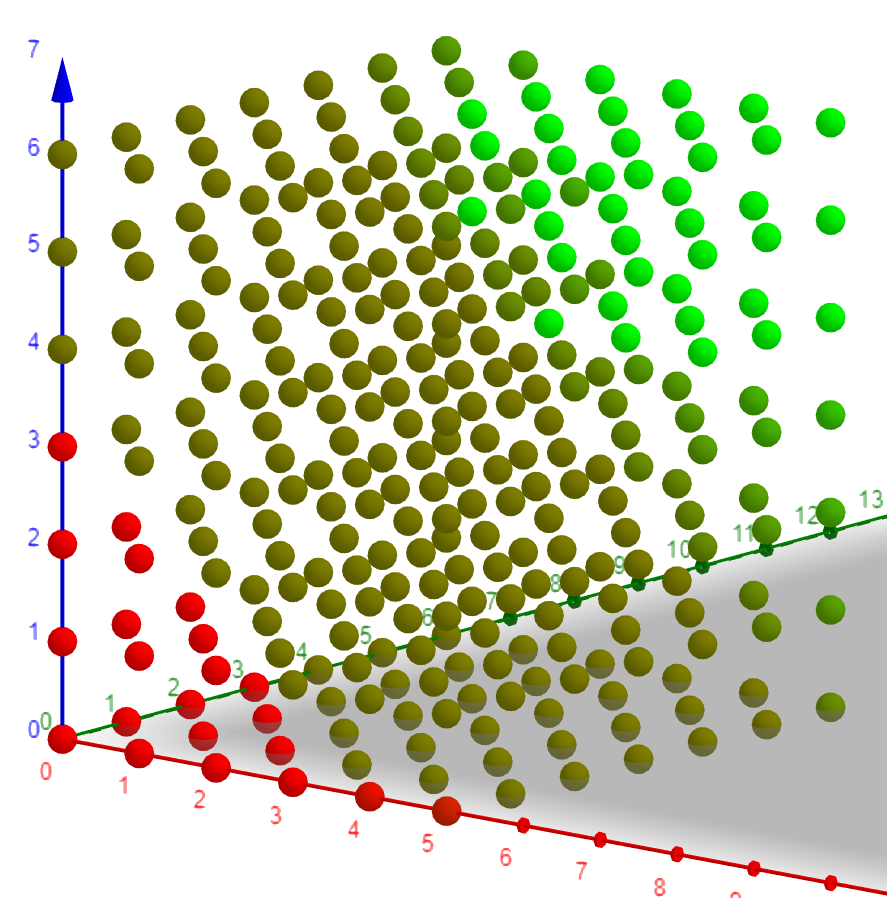
\includegraphics[width=20em]{cube.png}
\end{center}
Here, you can see that there are approximately diagonal thresholds where 
transitions between truckloads ordered occur. However, these aren't exact; 
for example even if you have 5 Alaska fridges but no other fridges, you should 
still order 2 truckloads. This is because Alaska fridges have a small profit margin
so it will be more profitable to have other fridge types as well.

Broadly, the optimal actions are grouped into 3 bunches---0, 1 and 2 truckloads. 
Most of the cases in each group will order the maximum possible but 
occasionally, you will want to order less due to the first paragraph in this section.

\section{Observations}
\begin{itemize}
    \item The limit of 8 fridges per type stored is a significant factor 
    in the runtime of the model. 
    \item Because the solution to communication 2 is so simple, the maximum 
    expected profit is actually linear as number of weeks increases. 
    Profit can be calculated as $\mathrm{number\ of\ weeks} \times \$1320.73$.
    \item However, comm 3 profit increases slightly faster than linear. This may 
    be because in later weeks it is possible that fridges are left over from 
    earlier weeks which can reduce later weeks' transport costs, increasing profit.

\end{itemize}

\part{Appendix}
We have included a file stochastic{\textunderscore}explorer.py to interactively 
explore the solution week by week. Communications 2 and 3 are supported.

\section{Usage}
\begin{enumerate}
    \item Place stochastic{\textunderscore}explorer.py is in the same folder as assignment{\textunderscore}dp.py.
    \item Run stochastic{\textunderscore}explorer.py.
    \item Type ``2'' or ``3'' for the communication you wish to consider. Press Enter.
    \item Once analysed, it will display the maximum expected profit and the fridges you should buy in the first week.
    \item Type in how many of each fridge you sold in that week.
    \item Your weekly and total profit will be displayed along with how many fridges you have stored for next week. Press Enter to continue. 
    \item Repeats from step 4 until you reach the end of the 4 weeks.
\end{enumerate}

\end{document}